\subsection{quantization}
	\begin{frame}\frametitle{sampling and quantization}\framesubtitle{quantization 1/2}
		\vspace{-3mm}
        \textbf{quantizer}: \linebreak
		continuous $\mapsto$ discrete (pre-defined set of allowed values)
        
        \pause
        \begin{itemize}
            \item   quantization is \textbf{non-linear}
            \item   quantization is \textbf{irreversible}
        \end{itemize}
		\begin{figure}
			\centering
				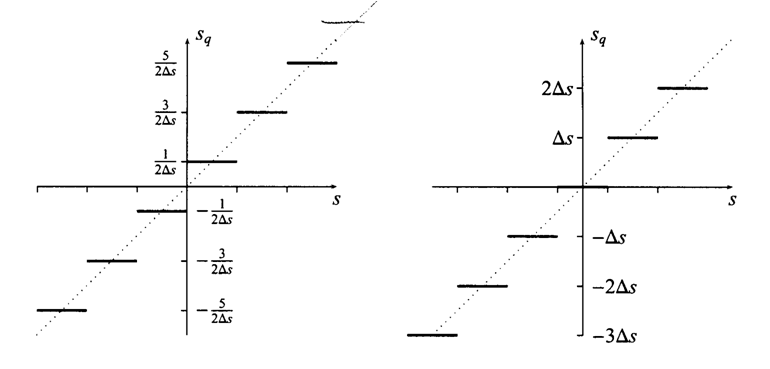
\includegraphics[scale=.4]{Graph/midtread-rise}
		\end{figure}
		\hspace{20mm} mid-rise \hspace{30mm} \only<2>{\textcolor{gtgold}}{mid-tread}
	\end{frame}
	
	\begin{frame}\frametitle{sampling and quantization}\framesubtitle{quantization 2/2}
		\begin{figure}
			\centering
				\includegraphics[scale=.8]{graph/quant}
		\end{figure}
		\pause
		\begin{itemize}
			\item	\textbf{number of quantization steps}: $\mathcal{M} = 16$
			\item	\textbf{word length (bits)}: \only<2>{?}\only<3->{$w = \log_2(\mathcal{M}) = \unit[4]{bit}$}
		\end{itemize}
	\end{frame}
	
	\begin{frame}\frametitle{sampling and quantization}\framesubtitle{quantization: wordlength \& number of steps}
		\begin{table}
			\centering
			\begin{tabular}{lcr}
			\hline
				$w$ & $\mathcal{M} = 2^w$ \\
			\hline
				1	&	2\\
				2	&	4\\
				4	&	16\\
				8	&	256\\
				12	&	4096\\
				16	&	65536\\
				20	&	1048576\\
				24	&	16777216\\
			\end{tabular}  
		\end{table}
	\end{frame}
	\begin{frame}\frametitle{sampling and quantization}\framesubtitle{quantization error 1/5}
		\begin{figure}
			\centering
			 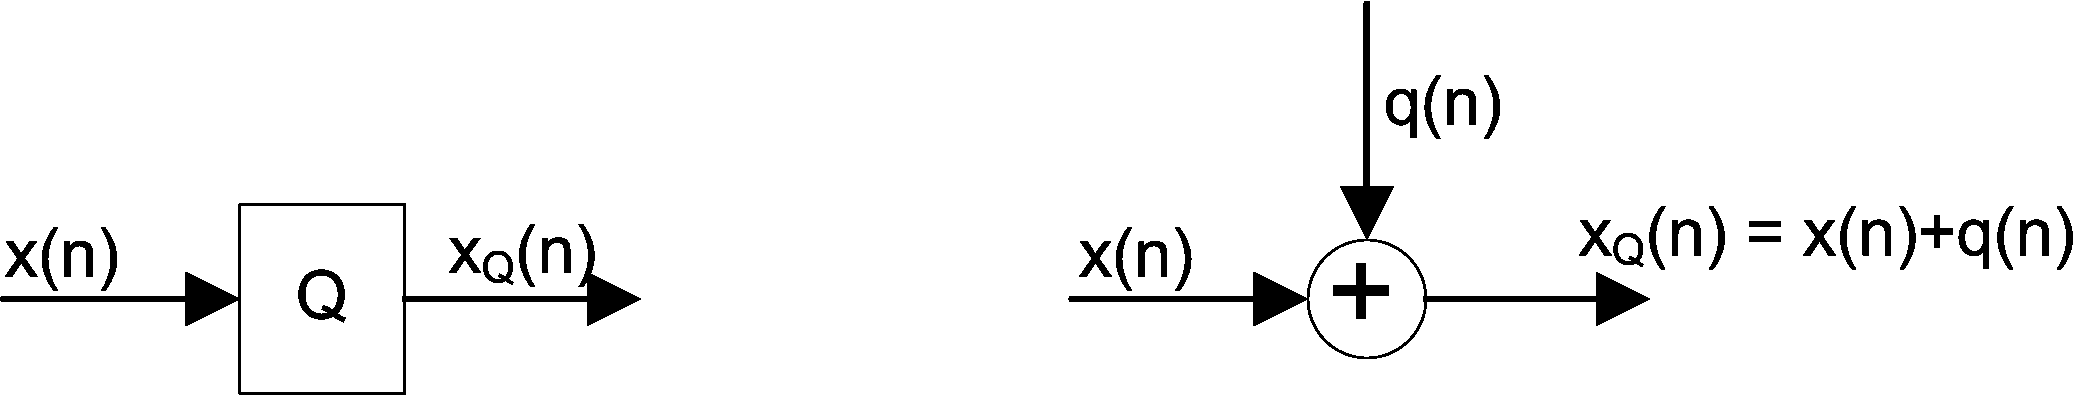
\includegraphics[scale=0.13]{Graph/Flowchart_Quantization}
		\end{figure}
		\begin{equation}
			q(i) = x(i) - x_{\mathrm{Q}}(i)
		\end{equation}
	\end{frame}		
	\begin{frame}\frametitle{sampling and quantization}\framesubtitle{quantization error 2/5}
		\vspace{-10mm}
		\begin{columns}
			\column{5cm}
			What is the maximum amplitude of the quantization error?
			
			\column{4cm}
			%\hspace{5mm}
			\begin{flushright}
				 
\includegraphics[scale=.08]{Graph/question-mark}
			\end{flushright}
		\end{columns}
		
		\pause
		\vspace{-3mm}
		\begin{figure}
			\centering
				\includegraphics[scale=.7]{\AcaGraph/quant}
		\end{figure}
	\end{frame}		
	\begin{frame}\frametitle{sampling and quantization}\framesubtitle{quantization error 3/5}
		\begin{figure}
			\centering
				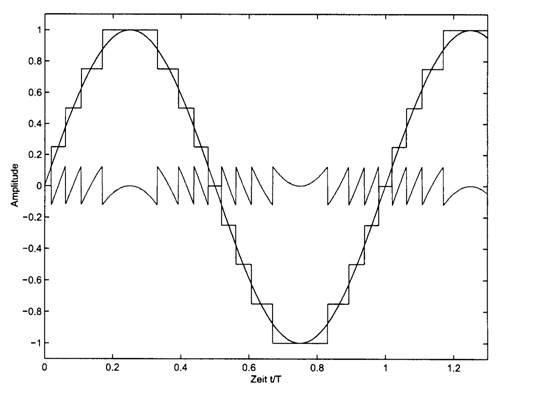
\includegraphics[scale=.6]{Graph/quant+quanterror}
		\end{figure}
	\end{frame}		
	\begin{frame}\frametitle{sampling and quantization}\framesubtitle{quantization error 4/5}
		\begin{figure}
			\centering
				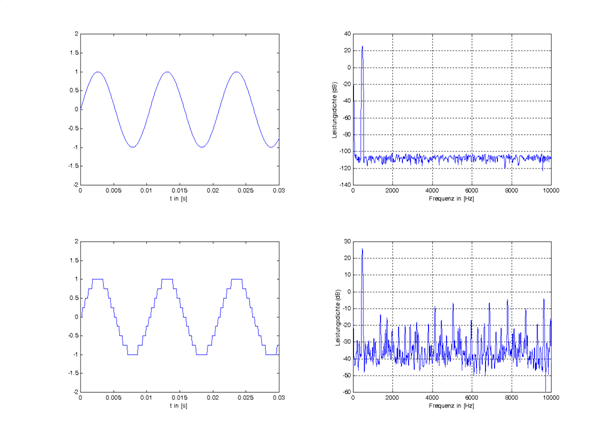
\includegraphics[scale=.6]{Graph/quanterror_spec}
		\end{figure}
	\end{frame}		
	\begin{frame}\frametitle{sampling and quantization}\framesubtitle{quantization error 5/5}
		\vspace{-10mm}
		\begin{columns}
			\column{.8\textwidth}
                assume small $\Delta$ compared to the signal amplitude:
                \begin{enumerate}
                    \item  What is the pdf of the quantization error?
                    \item  What is the shape of the magnitude spectrum of the quantization error?
                \end{enumerate}
			
			
			
			\column{.2\textwidth}
			%\hspace{5mm}
			\begin{flushright}
				 
\includegraphics[scale=.08]{Graph/question-mark}
			\end{flushright}
		\end{columns}
		
		\pause
		\vspace{-3mm}
    	\begin{figure}[!hbt]
			\begin{center}
			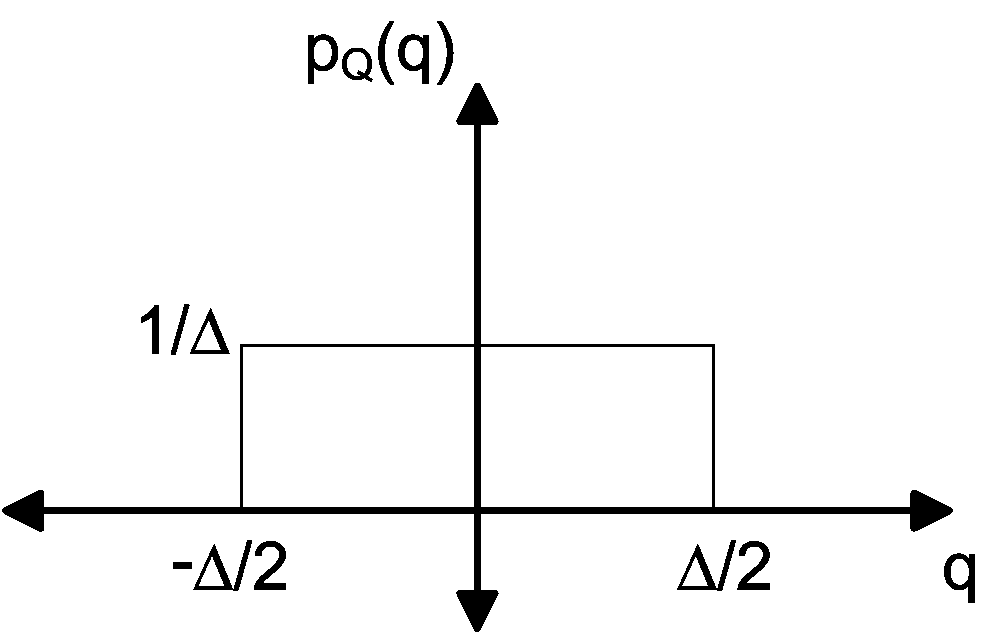
\includegraphics[scale=0.15]{Graph/QuantError_ADV}
			\end{center}
		\end{figure}
	\end{frame}
	\begin{frame}\frametitle{sampling and quantization}\framesubtitle{quantization: pdf of quant error}
        \vspace{-3mm}
        it can be shown that the pdf of the quantization error depends (without derivation)
        \begin{itemize}
            \item on the \textbf{variance of the input} signal in relation to the step size
            \item   on the \textbf{pdf of the input} signal
            \pause
            \item[$\rightarrow$]   will be \textbf{uniform for large values of} $\frac{\sigma_X}{\Delta}$
        \end{itemize}
    	\begin{figure}
			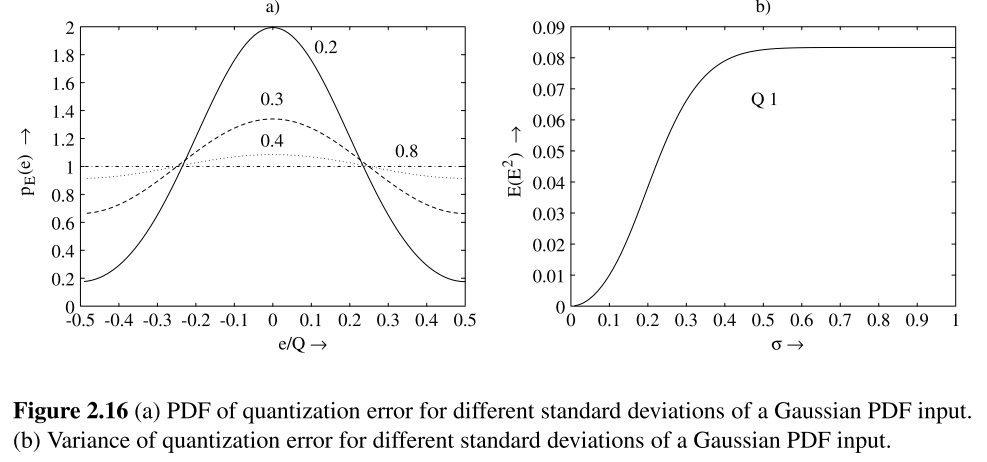
\includegraphics[scale=0.5]{Graph/pdfquanterr_variance}
		\end{figure}
	\end{frame}
	\begin{frame}\frametitle{sampling and quantization}\framesubtitle{quantization: audio examples}
		%\begin{table}
			%\begin{center}
				%\begin{tabular}{lcccccc}
				%\hline
					%$w$ & sine $x_Q(i)$ & sine $q(i)$ & speech $x_Q(i)$ & speech $q(i)$ & music $x_Q(i)$ & music $q(i)$ \\
				%\hline
				%\end{tabular}  
			%\end{center}
		%\end{table}
        \begin{footnotesize}
        \begin{itemize}
            \item[$w$]  $x_\mathrm{Q,sine}(i)$ \hspace{1mm} $q_\mathrm{sine}(i)$ \hspace{1mm} $x_\mathrm{Q,speech}(i)$ \hspace{1mm} $q_\mathrm{speech}(i)$ \hspace{1mm} $x_\mathrm{Q,music}(i)$ \hspace{1mm} $q_\mathrm{music}(i)$
            \item[$16$] \includeaudio{audio/sine_quant_16bit.mp3} \hspace{6mm} \includeaudio{audio/sine_quant_16bit_Q.mp3}  \hspace{4mm}
                     \includeaudio{audio/sqam_49_female_16bit.mp3} \hspace{8mm} \includeaudio{audio/sqam_49_female_16bit_Q.mp3} \hspace{7mm}
                     \includeaudio{audio/bigband_16bit.mp3} \hspace{7mm} \includeaudio{audio/bigband_16bit_Q.mp3} 

                \item[$12$] \includeaudio{audio/sine_quant_12bit.mp3} \hspace{6mm} \includeaudio{audio/sine_quant_12bit_Q.mp3}  \hspace{4mm}
                     \includeaudio{audio/sqam_49_female_12bit.mp3} \hspace{8mm} \includeaudio{audio/sqam_49_female_12bit_Q.mp3} \hspace{7mm}
                     \includeaudio{audio/bigband_12bit.mp3} \hspace{7mm} \includeaudio{audio/bigband_12bit_Q.mp3} 
                \item[$8$] \includeaudio{audio/sine_quant_8bit.mp3} \hspace{6mm} \includeaudio{audio/sine_quant_8bit_Q.mp3}  \hspace{4mm}
                     \includeaudio{audio/sqam_49_female_8bit.mp3} \hspace{8mm} \includeaudio{audio/sqam_49_female_8bit_Q.mp3} \hspace{7mm}
                     \includeaudio{audio/bigband_8bit.mp3} \hspace{7mm} \includeaudio{audio/bigband_8bit_Q.mp3} 
                \item[$6$] \includeaudio{audio/sine_quant_6bit.mp3} \hspace{6mm} \includeaudio{audio/sine_quant_6bit_Q.mp3}  \hspace{4mm}
                     \includeaudio{audio/sqam_49_female_6bit.mp3} \hspace{8mm} \includeaudio{audio/sqam_49_female_6bit_Q.mp3} \hspace{7mm}
                     \includeaudio{audio/bigband_6bit.mp3} \hspace{7mm} \includeaudio{audio/bigband_6bit_Q.mp3} 
                \item[$4$] \includeaudio{audio/sine_quant_4bit.mp3} \hspace{6mm} \includeaudio{audio/sine_quant_4bit_Q.mp3}  \hspace{4mm}
                     \includeaudio{audio/sqam_49_female_4bit.mp3} \hspace{8mm} \includeaudio{audio/sqam_49_female_4bit_Q.mp3} \hspace{7mm}
                     \includeaudio{audio/bigband_4bit.mp3} \hspace{7mm} \includeaudio{audio/bigband_4bit_Q.mp3} 
                \item[$2$] \includeaudio{audio/sine_quant_2bit.mp3} \hspace{6mm} \includeaudio{audio/sine_quant_2bit_Q.mp3}  \hspace{4mm}
                     \includeaudio{audio/sqam_49_female_2bit.mp3} \hspace{8mm} \includeaudio{audio/sqam_49_female_2bit_Q.mp3} \hspace{7mm}
                     \includeaudio{audio/bigband_2bit.mp3} \hspace{7mm} \includeaudio{audio/bigband_2bit_Q.mp3} 
        \end{itemize}
        \end{footnotesize}
    \end{frame}		
	
	\begin{frame}\frametitle{sampling and quantization}\framesubtitle{quality assessment of a quantizer: SNR}
        \begin{equation}\nonumber
            SNR = \frac{\text{signal energy}}{\text{noise energy}}
        \end{equation}
        \pause
			\begin{equation}\label{eq:snr}
				SNR = 10\cdot\log_{10}\left(\frac{W_{\mathrm{S}}}{W_{\mathrm{Q}}}\right)\; [dB] 
			\end{equation}
	\end{frame}		
	
	\begin{frame}\frametitle{sampling and quantization}\framesubtitle{quantization: SNR 1/2}
		\vspace{-5mm}
		\begin{columns}
			\column{6cm}
			What is the SNR of a quantized sinusoidal?
			\begin{equation}\nonumber
				SNR = 10\cdot\log_{10}\left(\frac{W_{\mathrm{S}}}{W_{\mathrm{Q}}}\right)\; [dB] 
			\end{equation}
			
			\hspace{3mm}use: $sin^2(t) = \frac{1-cos(2t)}{2}$
			
			\column{4cm}
			%\hspace{5mm}
			\begin{flushright}
				 
\includegraphics[scale=.08]{Graph/question-mark}
			\end{flushright}
		\end{columns}
		
		\pause
		\begin{eqnarray}
			W_S &=& \frac{A^2}{2} = \frac{(\Delta\cdot 2^{w-1})^2}{2}\\
			W_Q &=& \frac{\Delta^2}{12}\\
			\pause
			\frac{W_S}{W_Q} &=& \frac{3}{2}\cdot 2^{2w}
		\end{eqnarray}
	\end{frame}		
	\begin{frame}\frametitle{sampling and quantization}\framesubtitle{quantization: SNR 2/2}
		\only<1>{
        \begin{flushright}
			 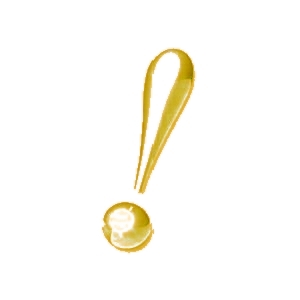
\includegraphics[scale=.25]{Graph/exclamation-mark}
		\end{flushright}
        }
		\begin{block}{Signal-to-Noise Ratio}
			\centering
			\begin{equation}
				SNR = 6.02\cdot w + c_{\mathrm{S}}\quad [dB]
			\end{equation}
			\begin{itemize}
				\item	every additional bit adds app.\ \unit[6]{dB} SNR
				\item	constant $c_{\mathrm{S}}$ depends on signal (scaling and PDF shape)
			\end{itemize}
		\end{block}
		\pause
		\begin{itemize}
			\item	square wave (full scale): $c_{\mathrm{S}} =  \unit[10.80]{dB}$
			\item	sinusoidal wave (full scale): $c_{\mathrm{S}} =  \unit[1.76]{dB}$
			\item	rectangular {PDF} (full scale): $c_{\mathrm{S}} =  \unit[0]{dB}$
			\item	Gaussian {PDF} (full scale = $4\sigma_{g}$): $c_{\mathrm{S}} =  \unit[-7.27]{dB}$
		\end{itemize}
	\end{frame}		
	\begin{frame}\frametitle{sampling and quantization}\framesubtitle{quantization: word length and SNR}
			\begin{table}
			\centering
				\begin{footnotesize}
					\begin{tabular}{lccc}
					\hline
						\textbf{w} & \textbf{$\Delta$} & \textbf{Max.\ Amp} & \textbf{theo.\ SNR} \\
					\hline
						8 (Int)	&	$\pm1$ & $0\ldots255$ & $\approx$\unit[48]{dB}\\
						16 (Int)	&	$\pm1$ & $-32768\ldots32767$ & $\approx$\unit[96]{dB}\\
						20 (Int)	&	$\pm1$ & $-524288\ldots524287$ & $\approx$\unit[120]{dB}\\
						24 (Int)	&	$\pm1$ & $-16777216\ldots16777215$ & $\approx$\unit[144]{dB}\\
					\hline
						32 (Float)	&	$\pm1.175\cdot10^{-38}$ & $\pm3.403\cdot10^{1038}$ & \unit[1529]{dB}\\
						64 (Float)	&	$\pm2.225\cdot10^{-308}$ & $\pm1.798\cdot10^{10308}$ & \unit[12318]{dB}\\
					\hline
					\end{tabular}  
				\end{footnotesize}
			\end{table}
	\end{frame}	
	
	\begin{frame}\frametitle{sampling and quantization}\framesubtitle{quantization: SNR and auditory sensation area}
	    \begin{figure}
			\centering
				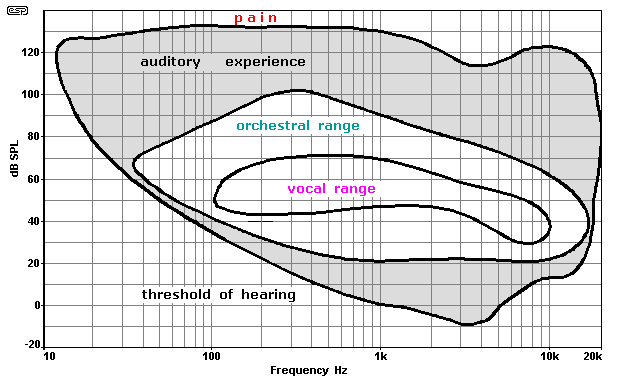
\includegraphics[scale=0.5]{Graph/hoerfeld}
		\end{figure}
	\end{frame}

	\begin{frame}\frametitle{sampling and quantization}\framesubtitle{quantization: SNR and signal scaling}
	    \begin{figure}
			\centering
				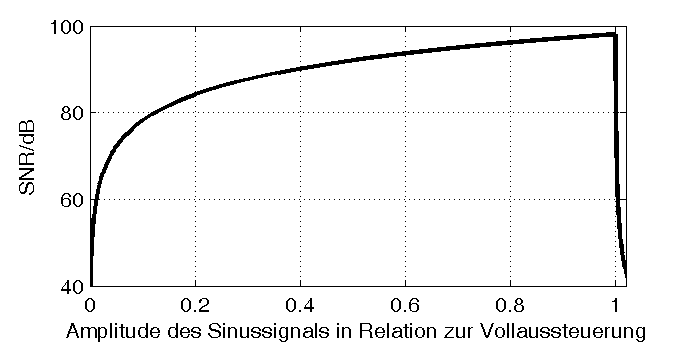
\includegraphics[scale=0.7]{Graph/snr}
		\end{figure}
	\end{frame}	
	
	%\begin{frame}\frametitle{sampling and quantization}\framesubtitle{quantization: clipping}
	    %\begin{figure}
	    	%\centering
				%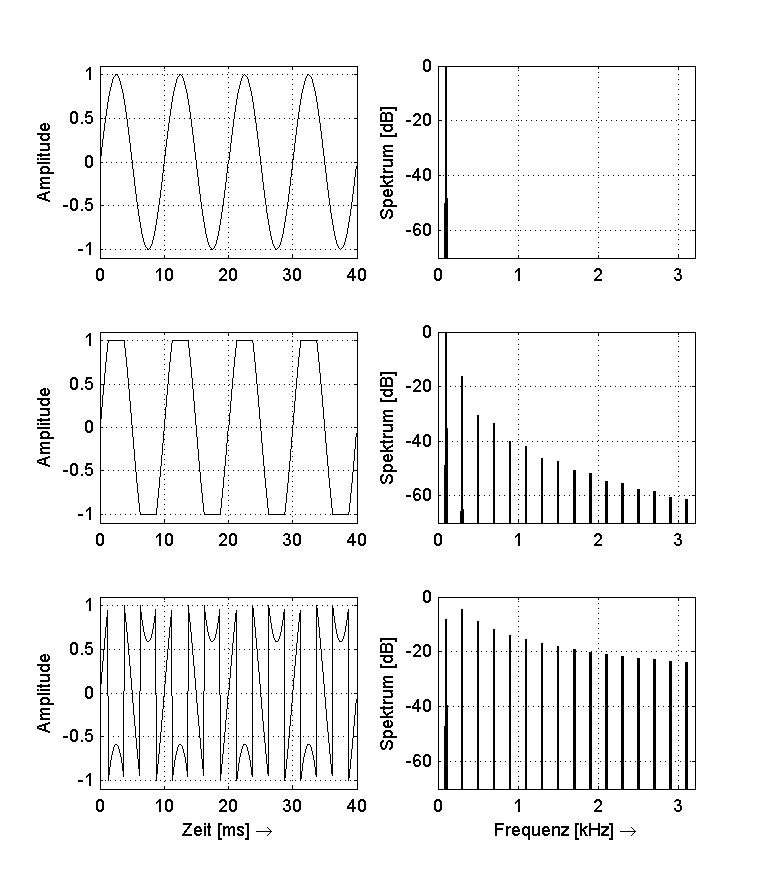
\includegraphics[scale=0.5]{Graph/Lerch14-11}
		%\end{figure}
	%\end{frame}	
	%
